\documentclass[border=15pt, multi, tikz]{standalone}
\usepackage{import}
\usepackage{ctex}% 中文支持
\usepackage{tikz}

\subimport{./}{init}
\usetikzlibrary{positioning}
\usetikzlibrary{3d} %for including external image
\usetikzlibrary{quotes,angles}
\usetikzlibrary{calc}
\usetikzlibrary{decorations.pathreplacing}

\def\DataColor{rgb:blue,5;white,5}
\def\ConvColor{rgb:yellow,5;red,2.5;white,5}
\def\ConvReluColor{rgb:yellow,5;red,5;white,5}
\def\PoolColor{rgb:red,1;black,0.3}
\def\PcColor{rgb:blue,5;red,2.5;white,5}
\def\PcSquashColor{rgb:blue,5;red,5;white,4}
\def\DcColor{rgb:blue,5;green,15}
% \def\SoftmaxColor{rgb:magenta,5;black,7}

\begin{document}
\begin{tikzpicture}
\tikzstyle{connection}=[ultra thick,every node/.style={sloped,allow upside down},draw=\edgecolor,opacity=0.7]
%%%%%%%%%%%%%%%%%%%%%%%%%%%%%%%%%%%%%%%%%%%%%%%%%%%%%%%%%%%%%%%%%%%%%%%%%%%%%%%%%%%%%%%%
%% Data
%%%%%%%%%%%%%%%%%%%%%%%%%%%%%%%%%%%%%%%%%%%%%%%%%%%%%%%%%%%%%%%%%%%%%%%%%%%%%%%%%%%%%%%%
\node[canvas is zy plane at x=0] (temp) at (-11,0,0) {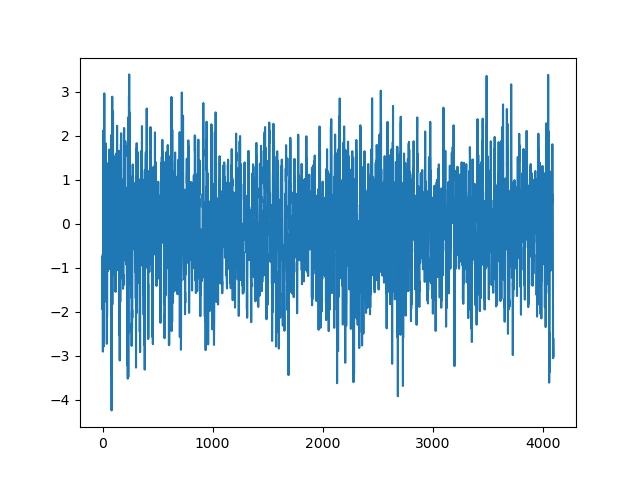
\includegraphics[width=6.4cm,height=4.8cm]{../DataInfo/signal.png}};
\node[] at (-9, 1, 0) {FFT};
\node[canvas is zy plane at x=0] (temp) at (-7.3,0,0) {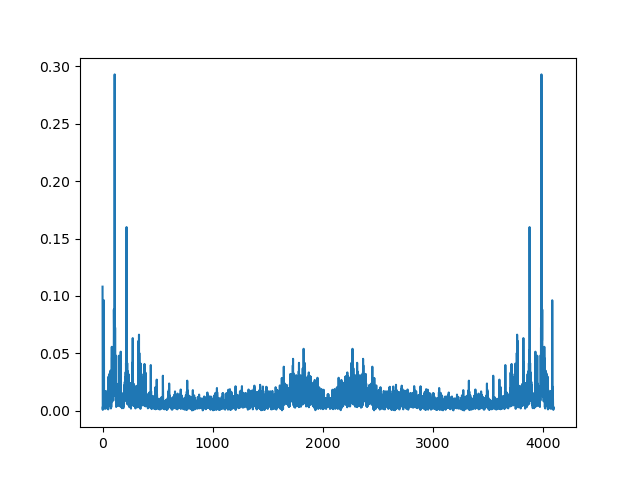
\includegraphics[width=6.4cm,height=4.8cm]{../DataInfo/signal_by_fft.png}};
\node[] at (-5.5, 1, 0) {Reshape};
\node[canvas is zy plane at x=0] (temp) at (-3.5,0,0) {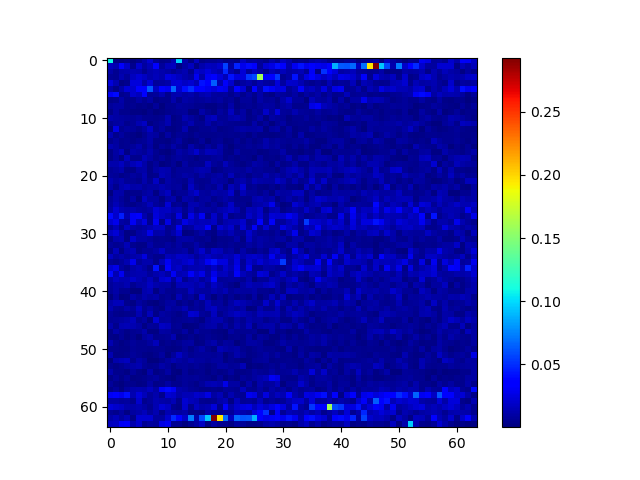
\includegraphics[width=6.4cm,height=4.8cm]{../DataInfo/input_image.png}};
% maxpool
\pic[shift={(-3.5,0,0)}] at (0,0,0) {Box={name=p,fill=\DataColor,opacity=0.5,height=32,width=2,depth=32}};
%%%%%%%%%%%%%%%%%%%%%%%%%%%%%%%%%%%%%%%%%%%%%%%%%%%%%%%%%%%%%%%%%%%%%%%%%%%%%%%%%%%%%%%%
%% Conv
%%%%%%%%%%%%%%%%%%%%%%%%%%%%%%%%%%%%%%%%%%%%%%%%%%%%%%%%%%%%%%%%%%%%%%%%%%%%%%%%%%%%%%%%
\pic[shift={(0,0,0)}] at (0,0,0) {RightBandedBox={name=cr,%
        xlabel={{"256", "256"}},ylabel=62,zlabel=62,fill=\ConvColor,bandfill=\ConvReluColor,%
        height=30,width=10,depth=30}};
% maxpool
\pic[shift={(1.5,0,0)}] at (cr-east) {Box={name=p,fill=\PoolColor,opacity=0.5,height=24,width=2,depth=24}};
% 文字
\node[] at (0, -5, 0) {Conv};
\node[] at (3, -4, 0) {MaxPool};
%%%%%%%%%%%%%%%%%%%%%%%%%%%%%%%%%%%%%%%%%%%%%%%%%%%%%%%%%%%%%%%%%%%%%%%%%%%%%%%%%%%%%%%%
%% Primary Capsule
%%%%%%%%%%%%%%%%%%%%%%%%%%%%%%%%%%%%%%%%%%%%%%%%%%%%%%%%%%%%%%%%%%%%%%%%%%%%%%%%%%%%%%%%
% primary capsule1
\pic[shift={(2,0,0)}] at (p-east) {RightBandedBox={name=pc1,%
        xlabel={{"32","32","32","32","32","32","32","32"}},ylabel=6,zlabel=6,fill=\ConvColor,bandfill=\ConvReluColor,%
        height=6,width={2,2,2,2,2,2,2,2},depth=6}};
%%%%%%%%%%
% primary capsule2
\pic[shift={(3,0,0)}] at (pc1-east) {RightBandedBox={name=pc2,
        fill=\PcColor,bandfill=\PcSquashColor,%
        height=8,width=3,depth=3}};
% 平移
\pic[shift={(3,0,4+2)}] at (pc1-east) {RightBandedBox={name=pc2-1,
        fill=\PcColor,bandfill=\PcSquashColor,%
        height=8,width=3,depth=3}};
\pic[shift={(3,0,4)}] at (pc1-east) {RightBandedBox={name=pc2-2,
        fill=\PcColor,bandfill=\PcSquashColor,%
        height=8,width=3,depth=3}};

\pic[shift={(3,0,-4)}] at (pc1-east) {RightBandedBox={name=pc2-3,
        fill=\PcColor,bandfill=\PcSquashColor,%
        height=8,width=3,depth=3}};
\pic[shift={(3,0,-4-2)}] at (pc1-east) {RightBandedBox={name=pc2-4,
        fill=\PcColor,bandfill=\PcSquashColor,%
        height=8,width=3,depth=3}};
% 省略号
\node[canvas is zy plane at x=0] (temp) at (12.5,0,2.2) {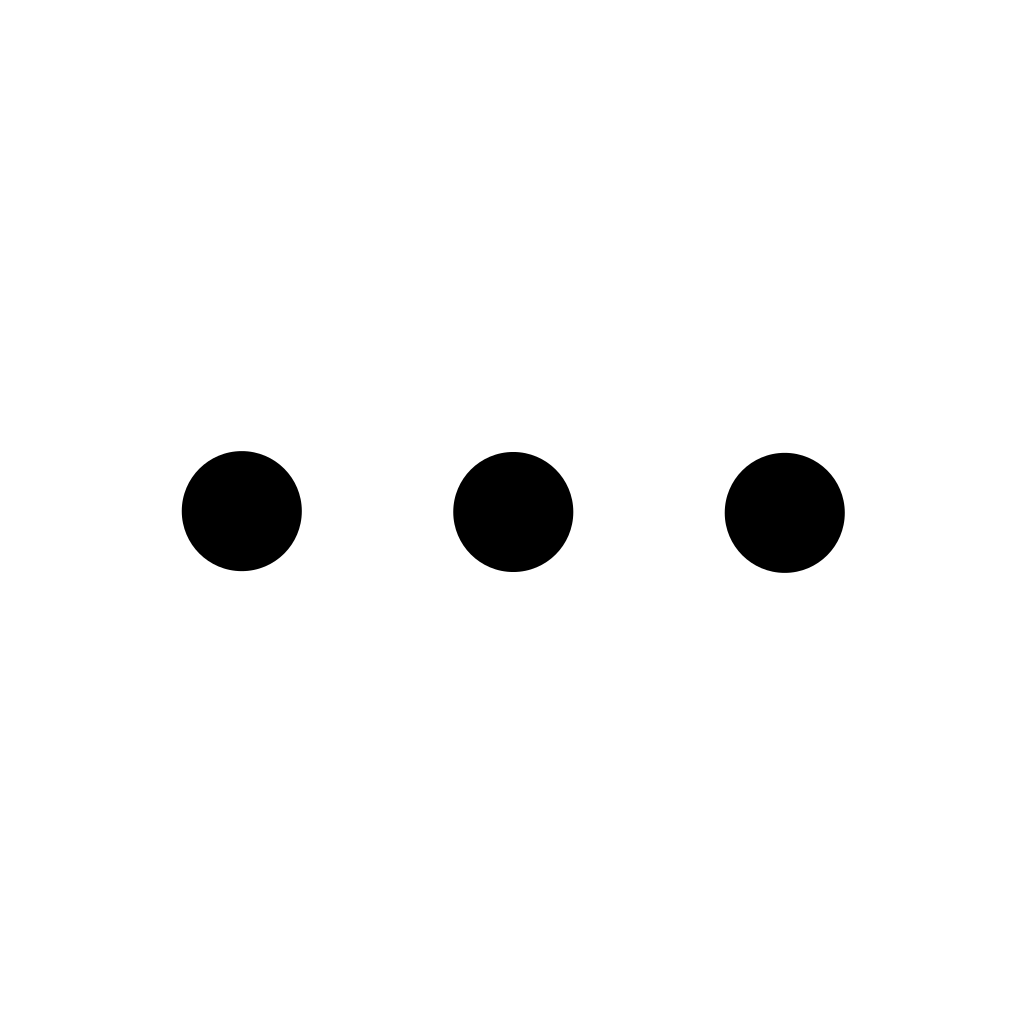
\includegraphics[width=2cm,height=2cm]{cellipsis.png}};
\node[canvas is zy plane at x=0] (temp) at (12.5,0,-1.7) {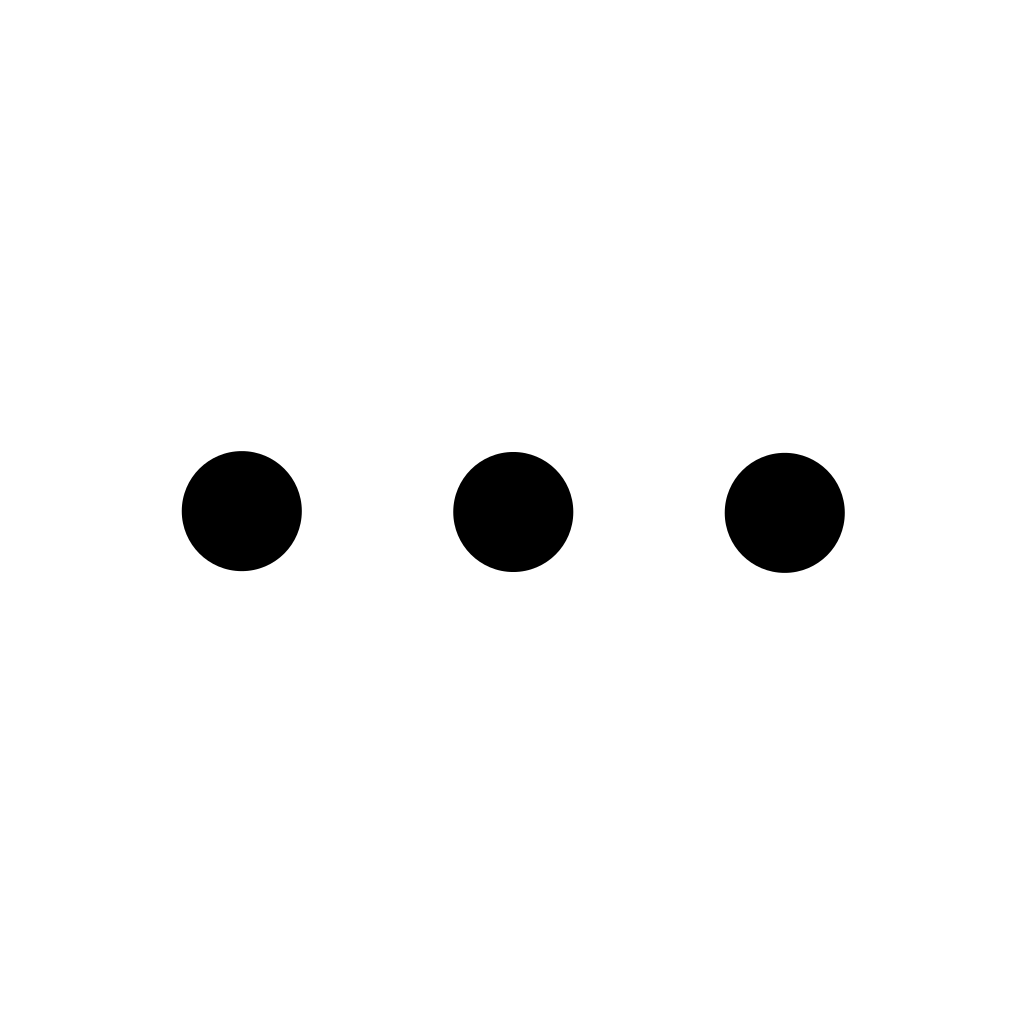
\includegraphics[width=2cm,height=2cm]{cellipsis.png}};
% 括号
\draw[decorate, decoration={brace, raise=15pt,amplitude=0.7cm},black!50] (13, -2.5, 0) -- (7, -2.5, 0);
% 文字
\node[] at (10, -4, 0) {Primary Capsule};
% 括号
\draw[decorate, decoration={brace, raise=15pt,amplitude=0.7cm},black!50] (10, -2.7, 0) -- (10, -2.7, -12);
% 文字
\node[rotate=45] at (6.8, -3.8, -11.5) {1152};
%%%%%%%%%%%%%%%%%%%%%%%%%%%%%%%%%%%%%%%%%%%%%%%%%%%%%%%%%%%%%%%%%%%%%%%%%%%%%%%%%%%%%%%%
%% Digit Capsule
%%%%%%%%%%%%%%%%%%%%%%%%%%%%%%%%%%%%%%%%%%%%%%%%%%%%%%%%%%%%%%%%%%%%%%%%%%%%%%%%%%%%%%%%
\pic[shift={(6,0,12)}] at (pc2-east) {Box={name=dc-1,fill=\DcColor,%
        height=3,width=3,depth=3}};
\pic[shift={(6,0,9)}] at (pc2-east) {Box={name=dc-2,fill=\DcColor,%
        height=3,width=3,depth=3}};
\pic[shift={(6,0,6)}] at (pc2-east) {Box={name=dc-3,fill=\DcColor,%
        height=3,width=3,depth=3}};
\pic[shift={(6,0,3)}] at (pc2-east) {Box={name=dc-4,fill=\DcColor,%
        height=3,width=3,depth=3}};
\pic[shift={(6,0,-3)}] at (pc2-east) {Box={name=dc-5,fill=\DcColor,%
        height=3,width=3,depth=3}};
\pic[shift={(6,0,-6)}] at (pc2-east) {Box={name=dc-6,fill=\DcColor,%
        height=3,width=3,depth=3}};
\pic[shift={(6,0,-9)}] at (pc2-east) {Box={name=dc-7,fill=\DcColor,%
        height=3,width=3,depth=3}};
\pic[shift={(6,0,-12)}] at (pc2-east) {Box={name=dc-8,fill=\DcColor,%
        height=3,width=3,depth=3}};
% 括号
\draw[decorate, decoration={brace, raise=15pt,amplitude=0.7cm},black!50] (19, 0, -12) -- (19, 0, 12);
% 文字
\node[] at (19, 0, 0) {Digit Capsule};
% \node[rotate=45] at (21.3, 0, 3) {8个一维向量代表8个类别出现的概率};
\node[rotate=45] at (21.3, 0, 3) {8 classes};
%%%%%%%%%%%%%%%%%%%%%%%%%%%%%%%%%%%%%%%%%%%%%%%%%%%%%%%%%%%%%%%%%%%%%%%%%%%%%%%%%%%%%%%%
%% Draw Arrow Connections
%%%%%%%%%%%%%%%%%%%%%%%%%%%%%%%%%%%%%%%%%%%%%%%%%%%%%%%%%%%%%%%%%%%%%%%%%%%%%%%%%%%%%%%%
\draw [connection]  (-10, 0, 0)        -- node {\midarrow} (-8.5, 0, 0);
\draw [connection]  (-7, 0, 0)        -- node {\midarrow} (-4, 0, 0);
\draw [connection]  (-2.5, 0, 0)        -- node {\midarrow} (cr-west);
\draw [connection]  (cr-east)        -- node {\midarrow} (p-west);
\draw [connection]  (p-east)        -- node {\midarrow} (pc1-west);
%%%%%%%%%%%%%%%%%%%%%%%%%%%%%%%%%%%%%%%%%%%%%%%%%%%%%%%%%%%%%%%%%%%%%%%%%%%%%%%%%%%%%%%%
%% Draw Connections
%%%%%%%%%%%%%%%%%%%%%%%%%%%%%%%%%%%%%%%%%%%%%%%%%%%%%%%%%%%%%%%%%%%%%%%%%%%%%%%%%%%%%%%%
% 循环变量
\foreach \from/\to in {pc2-1-east/dc-1-west, pc2-1-east/dc-2-west, pc2-1-east/dc-3-west, pc2-1-east/dc-4-west, pc2-1-east/dc-5-west, pc2-1-east/dc-6-west, pc2-1-east/dc-7-west, pc2-1-east/dc-8-west}
    \draw[->]  (\from) -- (\to);

\foreach \from/\to in {pc2-2-east/dc-1-west, pc2-2-east/dc-2-west, pc2-2-east/dc-3-west, pc2-2-east/dc-4-west, pc2-2-east/dc-5-west, pc2-2-east/dc-6-west, pc2-2-east/dc-7-west, pc2-2-east/dc-8-west}
    \draw[->]  (\from) -- (\to);
\foreach \from/\to in {pc2-east/dc-1-west, pc2-east/dc-2-west, pc2-east/dc-3-west, pc2-east/dc-4-west, pc2-east/dc-5-west, pc2-east/dc-6-west, pc2-east/dc-7-west, pc2-east/dc-8-west}
    \draw[->]  (\from) -- (\to);
\foreach \from/\to in {pc2-3-east/dc-1-west, pc2-3-east/dc-2-west, pc2-3-east/dc-3-west, pc2-3-east/dc-4-west, pc2-3-east/dc-5-west, pc2-3-east/dc-6-west, pc2-3-east/dc-7-west, pc2-3-east/dc-8-west}
    \draw[->]  (\from) -- (\to);
\foreach \from/\to in {pc2-4-east/dc-1-west, pc2-3-east/dc-2-west, pc2-4-east/dc-3-west, pc2-4-east/dc-4-west, pc2-4-east/dc-5-west, pc2-4-east/dc-6-west, pc2-4-east/dc-7-west, pc2-4-east/dc-8-west}
    \draw[->]  (\from) -- (\to);
%%%%%%%%%%%%%%%%%%%%%%%%%%%%%%%%%%%%%%%%%%%%%%%%%%%%%%%%%%%%%%%%%%%%%%%%%%%%%%%%%%%%%%%%
%% Draw Dotted Edges 
%%%%%%%%%%%%%%%%%%%%%%%%%%%%%%%%%%%%%%%%%%%%%%%%%%%%%%%%%%%%%%%%%%%%%%%%%%%%%%%%%%%%%%%%
\draw[densely dashed]
    (pc2-1-west)++(3, 3.7, 8) coordinate(a) -- (pc1-nearnortheast)
    (pc2-4-west)++(2, 1.3, 17.5) coordinate(b) -- (pc1-nearsoutheast)
    (pc2-4-west)++(-0.5, -1.9, -3) coordinate(c) -- (pc1-farsoutheast)
    (pc2-1-west)++(3.4, 3.7, -4.5) coordinate(d) -- (pc1-farnortheast)
    % (a)--(b)--(c)--(d)
    ;
%%%%%%%%%%%%%%%%%%%%%%%%%%%%%%%%%%%%%%%%%%%%%%%%%%%%%%%%%%%%%%%%%%%%%%%%%%%%%%%%%%%%%%%%
\end{tikzpicture}
\end{document}
